%2.	The paper should provide additional information on the estimation sample: Are the event-study models estimated within a fixed window? What happened to observations outside the window (included but not reported or binned-up)?


Thanks. Information on the estimation sample is now described in the data section and then provided in the footnote below each figure in the manuscript.

In the ENUSC data, the analytical sample includes the 47 municipalities surveyed in the ENUSC that were not treated in 2003 or earlier, the first year for which data are available. The sample period is restricted to 2003--2012 by two features of the data. First, the ENUSC is only available from 2003. Second, since all but one ENUSC municipality is eventually treated, the Callaway and Sant'Anna estimator cannot use already-treated municipalities as controls, and extending the sample beyond 2012---the last year in which an ENUSC municipality adopted the program---would leave only a single never-treated municipality as the comparison group. This results in an event study with a maximum of 5 pre-treatment and 7 post-treatment periods.\footnote{Some variables---such as trust in the police, police presence, or complaints about lack of police presence---are not available in every ENUSC wave, so the number of pre- and post-treatment periods may differ across event studies for these variables.} Note that since treatment adoption is staggered, not all municipalities contribute to the estimation of every pre- and post-treatment period. As a robustness check, we also estimate the main results using a balanced panel of municipalities, which is reported in Online Appendix C in the updated manuscript. We restrict the sample to municipalities that implemented \emph{Plan Cuadrante} between 2006 and 2009, enabling the construction of a symmetric window from $t-2$ to $t+3$. The resulting estimates are very similar to those from the main specification.


The administrative data are available for the full set of Chilean municipalities---reported crimes from 2002 to 2016 and arrests from 2005 to 2016. Because reported crime is available from 2002, the analytical sample for this outcome includes 292 municipalities: all municipalities that adopted \emph{Plan Cuadrante} from 2003 onward, together with all never-treated municipalities. Because arrests are only available from 2005, the corresponding analytical sample is restricted to 281 municipalities: all municipalities that adopted the program from 2005 onward, together with all never-treated municipalities. For symmetry with the ENUSC analysis, the main specification is nonetheless restricted to 5 pre-treatment and 7 post-treatment periods in both samples. We conduct here two robustness checks. First, we also estimate the effects using the full set of pre- and post-treatment periods available in each administrative sample and find consistent results. Second, we restrict the sample to municipalities that implemented \emph{Plan Cuadrante} between 2006 and 2009 and construct a symmetric window from $t-2$ to $t+3$. Once again, the resulting estimates are very similar to those from the main specification.

Below we reproduce the relevant paragraphs from the Data subsection of the updated manuscript, describing the construction of both analytical samples:

\begin{adjustwidth}{2em}{0em}
We combine administrative and survey data from \emph{Carabineros}, the Undersecretary for Crime Prevention, and the National Institute of Statistics (INE).

\emph{Carabineros} provided information on \emph{Plan Cuadrante} implementation, which we use to define treatment status across municipalities over time. The National Institute of Statistics granted access to the National Survey on Security and Crime (ENUSC), a repeated cross-section first conducted in 2003 and administered annually between October and December since 2005. The survey covers more than 25,000 households across 101 urban municipalities, collecting information on crime victimization, perceptions, trust in police, and household prevention measures over the previous 12 months.\footnote{The survey is administered to a randomly selected household member who must: a) live in the household, b) be 15 years or older, c) not be a domestic worker, and d) not have any disability preventing survey comprehension.}

Our empirical approach excludes always-treated municipalities \citep{Callaway}. Given ENUSC's first implementation in 2003 and absence in 2004, our main sample includes households from 46 urban municipalities that adopted \emph{Plan Cuadrante} between 2005 and 2012 plus one never-treated municipality.\footnote{This sample excludes municipalities adopting \emph{Plan Cuadrante} in 2013 as they are not covered by ENUSC. Also, there is only one never treated municipality covered by ENUSC.} The treated municipalities in this analytical sample account for approximately 27\% of Chile's population.

The Undersecretary for Crime Prevention provided data on the number of reported crimes (2002--2016) and arrests (2005--2016) for all municipalities. This comprehensive coverage allows us to expand the analytical sample: for reported crime, we include all municipalities adopting \emph{Plan Cuadrante} after 2002 together with never-treated municipalities, for a total of 292 municipalities; for arrests, the corresponding sample includes all post-2005 adopters and never-treated municipalities, for a total of 281 municipalities. The treated municipalities in these analytical samples account for over half of Chile's population.

The study period differs across the two data sources, as each covers a different time span and a different set of municipalities. For the ENUSC-based analysis, it is restricted to 2003--2012. The \citet{Callaway} estimator uses not-yet-treated and never-treated municipalities as the comparison group. Since only one municipality in the survey sample is never treated, extending the analysis beyond 2012---the last year in which a municipality surveyed in ENUSC adopts the program---would leave only that single never-treated unit as the comparison group for subsequent periods, making the estimates unreliable. The administrative data, by contrast, cover a large number of never-treated municipalities that can serve as controls throughout the full data period, allowing us to exploit the complete administrative coverage---2002--2016 for reported crime and 2005--2016 for arrests---and to include all municipalities adopting the program from 2003 to 2013, when the last municipality joins \emph{Plan Cuadrante}.

Together, the treated municipalities in our two analytical samples represent substantial shares of the Chilean population---approximately 27\% in the ENUSC-based analysis and over half in the administrative data analysis---and are geographically distributed across the country rather than clustered in a single region. Tables \ref{tab:sum_statsA2} and \ref{tab:sum_statsA3} in Online Appendix \ref{sec:appendixA} and Table \ref{tab:comparing_samples} and Figure \ref{fig:pcsp_maps} in Online Appendix \ref{sec:appendixB} provide a detailed characterization of the treated municipalities in each analytical sample relative to the average Chilean municipality.
\end{adjustwidth}

Note also the following footnote to Section 4 in the main manuscript:

\begin{adjustwidth}{2em}{0em}
Online Appendix Figure \ref{fig:admin_uncapped} reports the results for reported crime and arrests using the full set of post-treatment and pre-treatment periods, which are very similar to those presented here.
\end{adjustwidth}

and the following subsection of Online Appendix C, ``Effects of \emph{Plan Cuadrante} Using the Full Set of Post-treatment and Pre-treatment Periods'', which reports the first robustness check described above:

\begin{adjustwidth}{2em}{0em}
For symmetry with the ENUSC-based analysis, the event studies for reported crime and arrests reported in the main text are restricted to 5 pre-treatment and 7 post-treatment periods. Because the administrative data are available for the full set of Chilean municipalities and therefore include a much larger number of never-treated municipalities than the ENUSC sample, we can estimate these effects over a longer window without exhausting the pool of valid comparison units. Figure \ref{fig:admin_uncapped} reports the effects of \emph{Plan Cuadrante} on reported crime and arrests using the full set of post-treatment and pre-treatment periods rather than capping the event study to the 5 pre-treatment and 7 post-treatment periods used in the main specification. The results are very similar to those presented in Section \ref{main_results}.
\end{adjustwidth}

as well as the following subsection of Online Appendix C, ``Effects of \emph{Plan Cuadrante} using a Balanced Panel'', which reports the second robustness check described above for both analytical samples:

\begin{adjustwidth}{2em}{0em}
Figure \ref{fig:figureA6_bp} shows the effects of \emph{Plan Cuadrante} on the main outcomes, but estimated using a balanced panel of municipalities. For the ENUSC-based outcomes, this panel includes only municipalities that implemented the \emph{Plan Cuadrante} between 2006 and 2009, which allows the construction of a balanced panel from t-2 to t+3 (31 municipalities). For the administrative outcomes, the balanced panel comprises those municipalities observed over that same t-2 to t+3 window around their own adoption (94 for reported crime and 78 for arrests). The resulting estimates are very similar to those presented in the main document.
\end{adjustwidth}

\clearpage
\noindent\textbf{Other figures and tables referenced above:}
\vspace{0.5em}

{\renewcommand{\thetable}{A.2}
\begin{table}[H]
\centering
\caption{Summary Statistics -- ENUSC sample}
\label{tab:sum_statsA2}
\begin{threeparttable}
\begin{tabular}{l r r r r r}
\toprule
 & Mean & SD & Min & Max & N \\
\midrule
\multicolumn{6}{@{}l}{\textit{Household}} \\
\quad Socioeconomic status               & 3.58  & 0.73  & 1    & 5    & 99,298 \\
\quad Victimization                    & 0.26  & 0.44  & 0    & 1    & 99,298 \\
\quad Crime perception (neighborhood)  & 0.38  & 0.49  & 0    & 1    & 95,598 \\
\quad Crime perception (municipality)  & 0.66  & 0.48  & 0    & 1    & 96,794 \\
\quad Crime perception (country)       & 0.79  & 0.41  & 0    & 1    & 98,525 \\
\quad Trust in the police              & 0.44  & 0.50  & 0    & 1    & 51,445 \\
\quad Investment in security measures  & 0.21  & 0.40  & 0    & 1    & 99,298 \\
\quad \emph{Plan Cuadrante} (year)                  & 2007  & 1.85  & 2005 & 2012 & 97,847 \\
\addlinespace
\multicolumn{6}{@{}l}{\textit{Household member interviewed}} \\
\quad Female                      & 0.55  & 0.50  & 0  & 1  & 99,298 \\
\quad Age                         & 43.87 & 17.95 & 15 & 99 & 99,298 \\
\quad Primary school attendance   & 0.98  & 0.14  & 0  & 1  & 99,298 \\
\quad Secondary school attendance & 0.72  & 0.45  & 0  & 1  & 99,298 \\
\quad University attendance       & 0.20  & 0.40  & 0  & 1  & 99,298 \\
\bottomrule
\end{tabular}
\begin{tablenotes}[flushleft]
\footnotesize
\item Note: This table presents summary statistics from the ENUSC sample, covering the 47 municipalities used in the survey-based analysis (46 that adopted \emph{Plan Cuadrante} between 2005 and 2012 plus one never-treated municipality). Socioeconomic status is a 1 to 5 measure produced by ENUSC surveys and based on self-reported socioeconomic strata, being 1 the highest ranked and 5 the lowest. Crime perception is equal to 1 if the interviewed person reports that crime has increased in the last 12 months. The \emph{Plan Cuadrante} (year) row is computed over treated municipalities only.
\end{tablenotes}
\end{threeparttable}
\end{table}
}

\clearpage

{\renewcommand{\thetable}{A.3}
\begin{table}[H]
\centering
\caption{Summary Statistics -- Administrative municipality level sample}
\label{tab:sum_statsA3}
\begin{threeparttable}
\begin{tabular}{l r r r r r}
\toprule
 & Mean & SD & Min & Max & N \\
\midrule
\multicolumn{6}{@{}l}{\textit{Panel A. Reported-crime sample (292 municipalities)}} \\
\quad Reported crime (per 100k pop.)            & 1,732.39 & 1,036.68 & 0.00   & 11,434.40 & 4,371 \\
\quad Arrests (per 100k pop.)                   & 332.07   & 271.75   & 0.00   & 1,712.30  & 3,504 \\
\quad Poverty rate (\%)                         & 25.74    & 9.72     & 5.65   & 58.33     & 3,720 \\
\quad Pop.\ density (pop./km\textsuperscript{2}) & 63.51   & 140.47   & 0.09   & 1,109.58  & 4,065 \\
\quad \emph{Plan Cuadrante} (year)                     & 2010     & 2.82     & 2003   & 2013      & 1,440 \\
\addlinespace
\multicolumn{6}{@{}l}{\textit{Panel B. Arrests sample (281 municipalities)}} \\
\quad Reported crime (per 100k pop.)            & 1,684.74 & 1,014.67 & 0.00   & 11,434.40 & 4,209 \\
\quad Arrests (per 100k pop.)                   & 313.21   & 251.23   & 0.00   & 1,712.30  & 3,372 \\
\quad Poverty rate (\%)                         & 26.01    & 9.72     & 5.65   & 58.33     & 3,570 \\
\quad Pop.\ density (pop./km\textsuperscript{2}) & 57.90   & 127.30   & 0.09   & 1,109.58  & 3,900 \\
\quad \emph{Plan Cuadrante} (year)                     & 2010     & 2.26     & 2006   & 2013      & 1,275 \\
\bottomrule
\end{tabular}
\begin{tablenotes}[flushleft]
\footnotesize
\item Note: The table reports municipality-level summary statistics for the two administrative estimation samples used in the paper. Panel A covers the 292 municipalities in the reported-crime sample (municipalities adopting \emph{Plan Cuadrante} from 2003 onward plus never-treated); Panel B the 281 municipalities in the arrests sample (adopters from 2006 onward plus never-treated --- municipalities adopting in 2005 are excluded because arrest data begin that year, leaving no pre-treatment period). Reported crime and arrests are measured per 100,000 inhabitants over 2002--2016 and 2005--2016, respectively. Minimum reported crime and arrests of zero correspond to tiny, remote never-treated comunas (e.g., Juan Fernández, Cabo de Hornos). The \emph{Plan Cuadrante} (year) row is computed over treated municipalities only. Data from the Undersecretary for Crime Prevention.
\end{tablenotes}
\end{threeparttable}
\end{table}
}

\clearpage

{\renewcommand{\thefigure}{B.1}
\begin{figure}[h!]
    \centering
    \caption{Geographic Distribution of \emph{Plan Cuadrante}}
    \label{fig:pcsp_maps}
    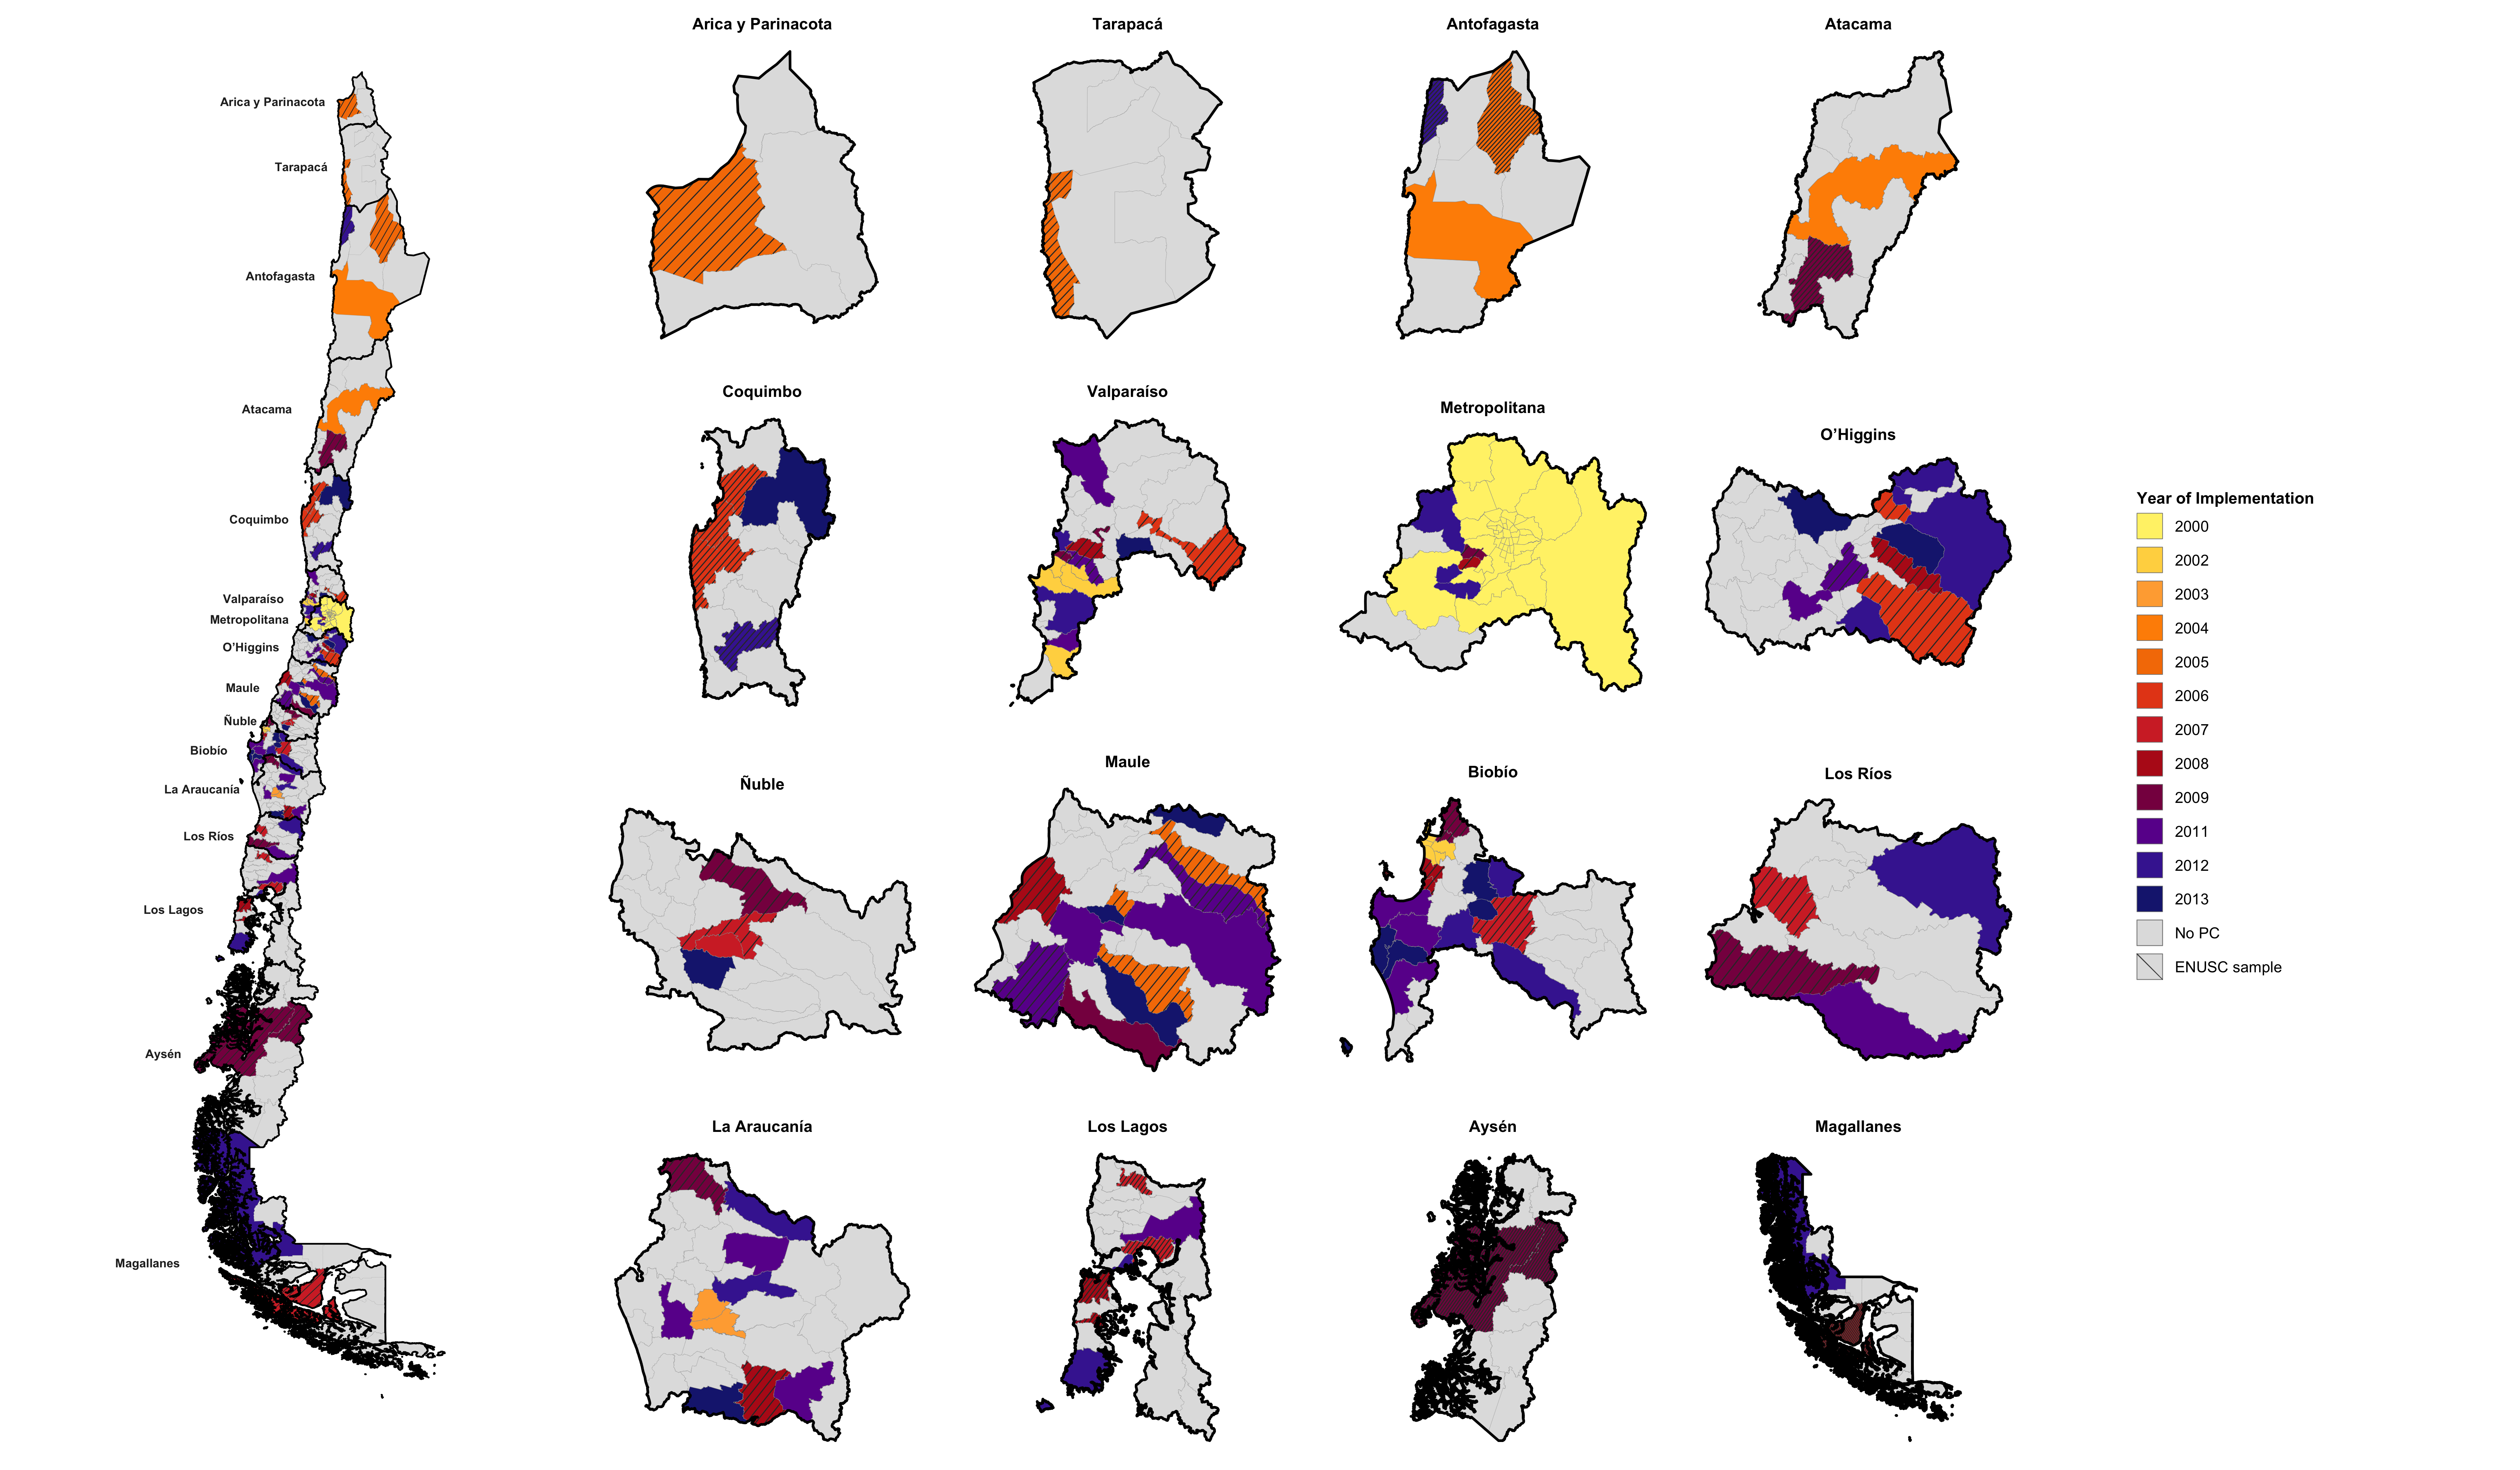
\includegraphics[width=\textwidth]{../manuscript/Graphs/mapa_PCSP_Chile_combinado.png}
    \begin{minipage}{0.95\textwidth}
    \footnotesize
    Notes: This figure shows the spatial rollout of \emph{Plan Cuadrante} across Chilean municipalities. The national map (left) is displayed alongside the 16 regional maps (right) for closer inspection. The color of each treated municipality indicates its year of program adoption, ranging from 2000 (lightest) to 2013 (darkest), following the legend. Municipalities shown in light grey were never treated under PC. Diagonal hatching identifies the 46 treated municipalities in the analytical sample used to estimate the effects on ENUSC outcomes.
    \end{minipage}
\end{figure}
}

\clearpage

{\renewcommand{\thetable}{B.1}
\begin{table}[H]
\caption{Baseline characteristics by subsample}
\label{tab:comparing_samples}
\begin{center}
\resizebox{\textwidth}{!}{
\begin{threeparttable}
\begin{tabular}{l cccccc}
\toprule
&  & \multicolumn{4}{c}{PC municipalities}  & \\
\cmidrule(lr){3-6}
& (1) & (2) & (3) & (4) & (5) & (6) \\
& All & All PC & Always- & Treated & Treated & Never- \\
& municipalities & municipalities & treated & ENUSC & admin.\ data & treated \\
\midrule
Reported crime (per 100k pop.) &     1,650.23 &     2,132.29 &     2,437.25 &     2,202.06 &     1,976.59 &     1,282.47 \\
Arrests (per 100k pop.)        &       267.62     &       442.08     &       606.01     &       459.05     &       358.11     &       134.11     \\
Poverty rate (\%)              &        23.73     &        20.50     &        14.88     &        21.73     &        23.96     &        26.82     \\
Pop.\ density (pop./km$^2$)   &       870.28 &     1,904.14 &     4,593.32 &       215.52 &       134.50 &        27.02 \\
Population                     &    57,857.22         &   117,975.43         &   187,558.74         &   113,079.74         &    81,532.84         &    11,612.44         \\
\midrule
Municipalities                 &          346            &          150            &           58            &           46            &           96            &          196            \\
\bottomrule
\end{tabular}
\begin{tablenotes}[flushleft]
\footnotesize{\item Note: Reported crime, poverty rate, population density, and population are measured as of 2003; arrests are measured as of 2005, the first year for which arrest data are available. Column (1) includes all municipalities in Chile. Column (2) includes all PC municipalities. Column (3) restricts to municipalities that adopted \emph{Plan Cuadrante} before 2005, the always-treated in our sample, which are therefore excluded from our estimation samples (as depicted in Figure 1, panel (a)). Column (4) restricts to treated municipalities in the analytical sample using the ENUSC data. Column (5) restricts to treated municipalities included in the analytical sample using the administrative data. Column (6) includes never-treated municipalities.}
\end{tablenotes}
\end{threeparttable}}
\end{center}
\end{table}
}

\clearpage

{\renewcommand{\thefigure}{C.8}
\begin{figure}[h!]
    \centering
    \caption{Effects of \emph{Plan Cuadrante} on Reported Crime and Arrests Using the Full Set of Post-treatment and Pre-treatment Periods}
    \label{fig:admin_uncapped}
    \begin{subfigure}{0.495\textwidth}
        \centering
        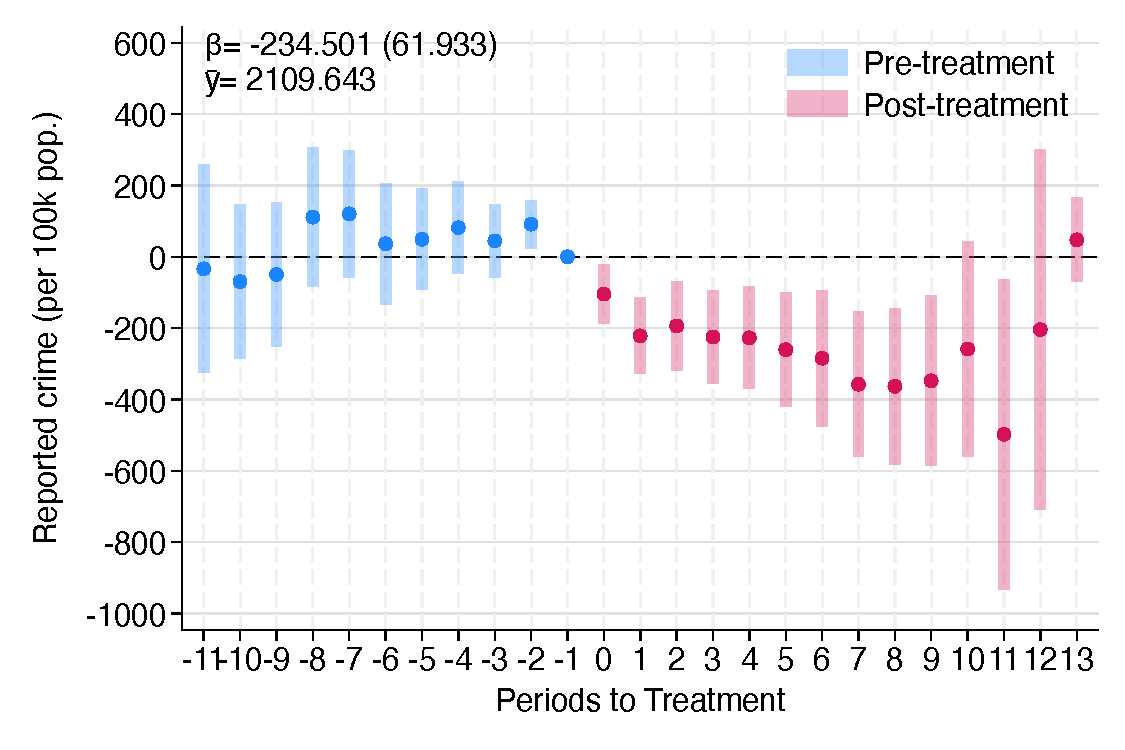
\includegraphics[width=0.98\textwidth]{../manuscript/Graphs/totalreportedcrime_allcomunas_uncapped.pdf}
        \caption{Reported crime per 100k inhabitants}
    \end{subfigure}%
    ~
    \begin{subfigure}{0.495\textwidth}
    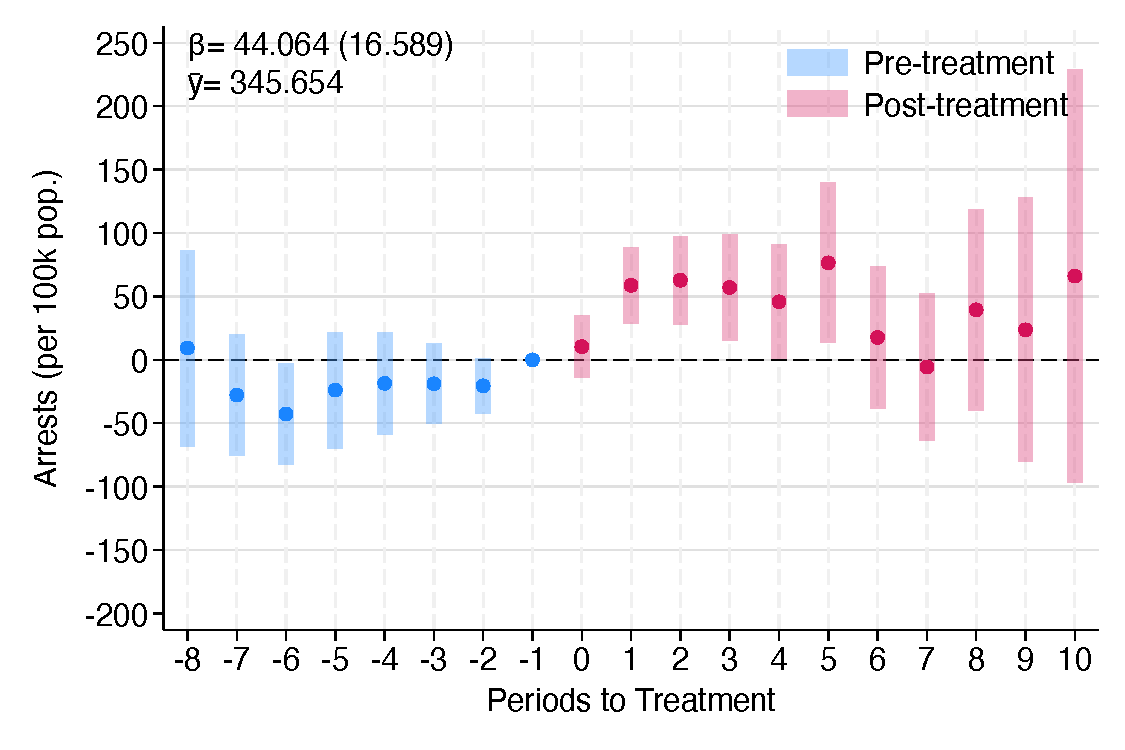
\includegraphics[width=0.98\textwidth]{../manuscript/Graphs/totalarrestscrime_allcomunas_uncapped.pdf}
        \caption{Arrests per 100k inhabitants}
    \end{subfigure}
    \begin{minipage}{\textwidth}
    \footnotesize
   Notes: This figure shows the dynamic effects of \emph{Plan Cuadrante} on the number of crimes reported to the police in the municipality per 100,000 inhabitants (panel a) and on the number of arrests in the municipality per 100,000 inhabitants (panel b), using administrative data. The estimation is conducted using the procedure developed in \citet{Callaway} for difference-in-differences with staggered treatment adoption. The dots in the figure represent the estimated coefficients and the bars behind them 95\% confidence intervals. Standard errors are clustered at the municipality level using the wild bootstrapping procedure. The pooled effect and the mean outcome before the introduction of the treatment are also presented in each panel. Unlike Figure \ref{fig:figure02} in the main text, we do not cap the event study to the same 5 pre-treatment and 6 post-treatment periods used for symmetry with the ENUSC-based analysis. Instead, we exploit the full set of post-treatment and pre-treatment periods. Panel (a) includes 4,371 observations and panel (b) 3,372 observations.
    \end{minipage}
\end{figure}
}

\clearpage

{\renewcommand{\thefigure}{C.7}
\begin{figure}[h!]
    \centering
    \caption{Effects of \emph{Plan Cuadrante} Using a Balanced Panel of Municipalities}
    \label{fig:figureA6_bp}
    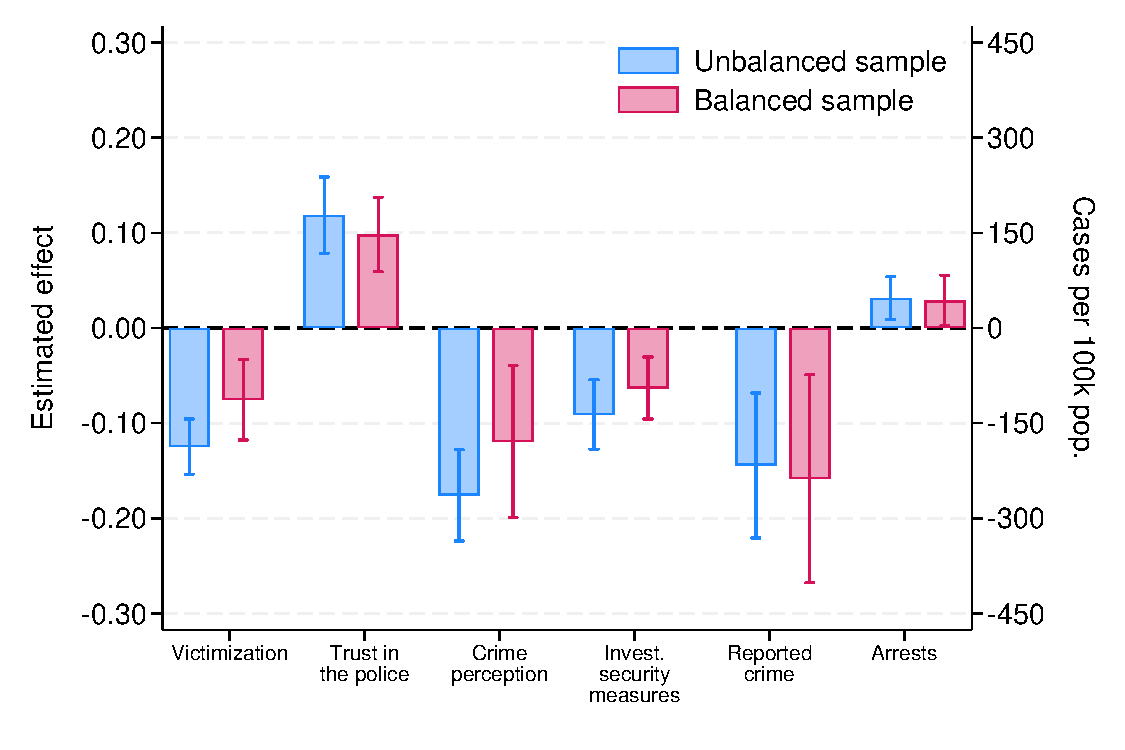
\includegraphics[width=0.8\textwidth]{../manuscript/Graphs/results_crime_balanced_combined.pdf}
    \\[10pt]
    \begin{minipage}{0.99\textwidth}
    \footnotesize Notes: The figure reports the effects of \emph{Plan Cuadrante} on different measures of police effectiveness using the main analytical sample (unbalanced, blue bars) and a balanced panel of municipalities observed over the full event-study window from $t-2$ to $t+3$ (red bars). For the ENUSC sample the balanced panel consists of the 31 municipalities that implemented \emph{Plan Cuadrante} between 2006 and 2009; for the administrative municipality-level sample it consists of 94 municipalities for reported crime and 78 municipalities for arrests. The bars represent the average post-treatment effect estimated with the difference-in-differences estimator developed in \citet{Callaway}, and the whiskers the 95\% confidence intervals; standard errors are clustered at the municipality level. Victimization is the probability of household victimization in the last 12 months; reported crime is the number of crimes reported to the police in the municipality per 100,000 inhabitants; arrests is the number of arrests per 100,000 inhabitants; trust in the police is the probability of reporting high trust in the police; crime perception is the probability of perceiving an increase in crime; and investment in security measures is the probability of adopting security measures in the last twelve months. Reported crime and arrests (administrative data) are read on the right axis; all other outcomes, from the ENUSC survey, are read on the left axis.
    \end{minipage}
\end{figure}
}

\clearpage

